\chapter{Introduction}

In the recent years, from late 2005, clocks’ speeds haven’t advanced anymore. Instead, core counts have increased at the pace clock speed used to, and that has affected more and more programmers. As programmers started migrating from single core to multicore architectural programming, many problems arose.

One of the most difficult parts of multi-threaded programming is when programmers need to handle critical sections (A critical section of a multithreaded program is a section of code where shared data are accessed by the multiple threads) which are responsible for causing data races and are also one of the reasons for causing deadlocks. Data races occur due to incorrect or no synchronization of the threads in the programs.

In order to avoid data races, synchronization is achieved by using lock/unlock mechanism (semaphores, monitors, pthread\_mutex, etc.) to limit a thread’s concurrent access to shared resources, if it is being used by other thread. To resolve the issue of manually handling each and every critical section or to debug large programs with synchronization bugs we are proposing an idea with which we identify critical sections which may cause data races, and avoid them by introducing proper synchronizations.
\newpage
\section{Background}
In multithreaded programs, we often need to handle cases where critical sections exist, as the programs are at risk of producing unexpected outputs. This is done by introducing locking mechanisms so that only one thread may alter the data at once. This is necessary to avoid race conditions, which generally lead to unexpected results if the locking mechanism doesn't exist.
\subsection{Multithreading}

In computer science, a thread of execution is the smallest sequence of programmed instructions that can be managed independently by an operating system scheduler. A thread is a light-weight process. The implementation of threads and processes differs from one operating system to another, but in most cases, a thread is contained inside a process. Multiple threads can exist within the same process and share resources such as memory, while different processes do not share these resources. In particular, the threads of a process share the latter's instructions (its code) and its context (the values that its variables reference at any given moment).
On a single processor, multithreading generally occurs by time-division multiplexing (as in multitasking): the processor switches between different threads. This context switching generally happens frequently enough that the user perceives the threads or tasks as running at the same time. On a multiprocessor or multi-core system, threads can be truly concurrent, with every processor or core executing a separate thread simultaneously[9].

Many modern operating systems directly support both time-sliced and multiprocessor threading with a process scheduler. The kernel of an operating system allows programmers to manipulate threads via the system call interface. Some implementations are called a kernel thread, whereas a lightweight process (LWP) is a specific type of kernel thread that shares the same state and information [9].
\begin{figure}[H]
\centering
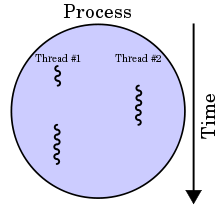
\includegraphics[scale=0.6]{threads.png}
\caption{Threads}
\label{<<Label>>}
\end{figure}

Thread-safeness:

Thread-safeness: in a nutshell, refers an application's ability to execute multiple threads simultaneously without "clobbering" shared data or creating "race" conditions.
For example, suppose that your application creates several threads, each of which makes a call to the same library routine:
This library routine accesses/modifies a global structure or location in memory.
As each thread calls this routine it is possible that they may try to modify this global structure/memory location at the same time.
If the routine does not employ some sort of synchronization constructs to prevent data corruption, then it is not thread-safe.[6]
\\
\begin{figure}[H]
\centering
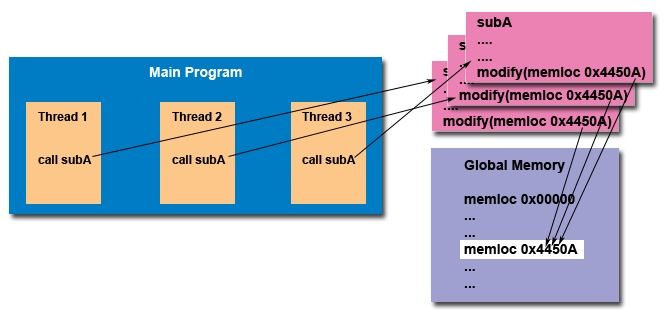
\includegraphics[scale=0.5]{multithreading.jpg}
\caption{Multithreading}
\label{<<Label>>}
\end{figure}
The implication to users of external library routines is that if you aren't 100 percent certain the routine is thread-safe, then you take your chances with problems that could arise.
Recommendation: Be careful if your application uses libraries or other objects that don't explicitly guarantee thread-safeness. When in doubt, assume that they are not thread-safe until proven otherwise. This can be done by "serializing" the calls to the uncertain routine, etc [6].

Shared Memory Model:

All threads have access to the same global, shared memory
Threads also have their own private data
Programmers are responsible for synchronizing access (protecting) globally shared data [6].

\begin{figure}[H]
\centering
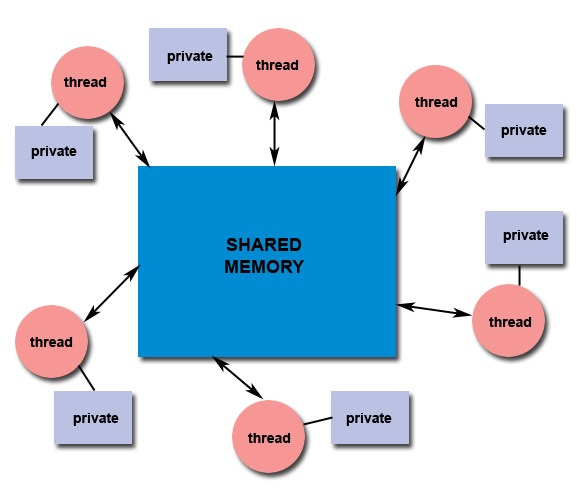
\includegraphics[scale=0.45]{shared.jpg}
\caption{Shared Memory}
\label{<<Label>>}
\end{figure}

\subsection{POSIX thread (pthread) libraries}
The POSIX thread libraries are a standards based thread API for C/C++. It allows one to spawn a new concurrent process flow. It is most effective on multi-processor or multi-core systems where the process flow can be scheduled to run on another processor thus gaining speed through parallel or distributed processing. Threads require less overhead than "forking" or spawning a new process because the system does not initialize a new system virtual memory space and environment for the process. While most effective on a multiprocessor system, gains are also found on uniprocessor systems which exploit latency in I/O and other system functions which may halt process execution. (One thread may execute while another is waiting for I/O or some other system latency.) 

Parallel programming technologies such as MPI and PVM are used in a distributed computing environment while threads are limited to a single computer system. All threads within a process share the same address space. A thread is spawned by defining a function and its arguments which will be processed in the thread. The purpose of using the POSIX thread library in your software is to execute software faster.

The subroutines which comprise the Pthreads API can be informally grouped into four major groups:
\begin{itemize}
\item Thread management: Routines that work directly on threads - creating, detaching, joining, etc. They also include functions to set/query thread attributes (joinable, scheduling etc.)
\\Creating and Terminating Threads:
\begin{itemize}
\item pthread\_create (thread, attr, start\_routine, arg)
\item pthread\_exit (status)
\item pthread\_cancel (thread)
\item pthread\_attr\_init (attr)
\item pthread\_attr\_destroy (attr)
\end{itemize}

\item Mutexes: Routines that deal with synchronization, called a "mutex", which is an abbreviation for "mutual exclusion". Mutex functions provide for creating, destroying, locking and unlocking mutexes. These are supplemented by mutex attribute functions that set or modify attributes associated with mutexes.
\\Mutex Variables:
\begin{itemize}
\item pthread\_mutex\_init (mutex, attr)
\item pthread\_mutex\_destroy (mutex)
\item pthread\_mutexattr\_init (attr)
\item pthread\_mutexattr\_destroy (attr)
\end{itemize} 

\item Condition variables: Routines that address communications between threads that share a mutex. Based upon programmer specified conditions. This group includes functions to create, destroy, wait and signal based upon specified variable values. 
\\Condition variable:
\begin{itemize}
\item pthread\_cond\_init (condition, attr)
\item pthread\_cond\_destroy (condition)
\item pthread\_condattr\_init (attr)
\item pthread\_condattr\_destroy (attr)
\end{itemize}

\item Synchronization: Routines that manage read / write locks and barriers.
\begin{itemize}
\item pthread\_mutex\_lock (mutex)
\item pthread\_mutex\_trylock (mutex)
\item pthread\_mutex\_unlock (mutex)
\item pthread\_cond\_wait (condition, mutex)
\item pthread\_cond\_signal (condition)
\end{itemize}
\end{itemize}


\subsection{Critical Section}
In concurrent programming, a critical section is a piece of code that accesses a shared resource (data structure or device) that must not be concurrently accessed by more than one thread of execution. A critical section will usually terminate in fixed time, and a thread, task, or process will have to wait for a fixed time to enter it (aka bounded waiting).

By carefully controlling which variables are modified inside and outside the critical section, concurrent access to that state is prevented. A critical section is typically used when a multi-threaded program must update multiple related variables without a separate thread making conflicting changes to that data. In a related situation, a critical section may be used to ensure a shared resource, for example a printer, can only be accessed by one process at a time.
\begin{figure}[H]
\centering
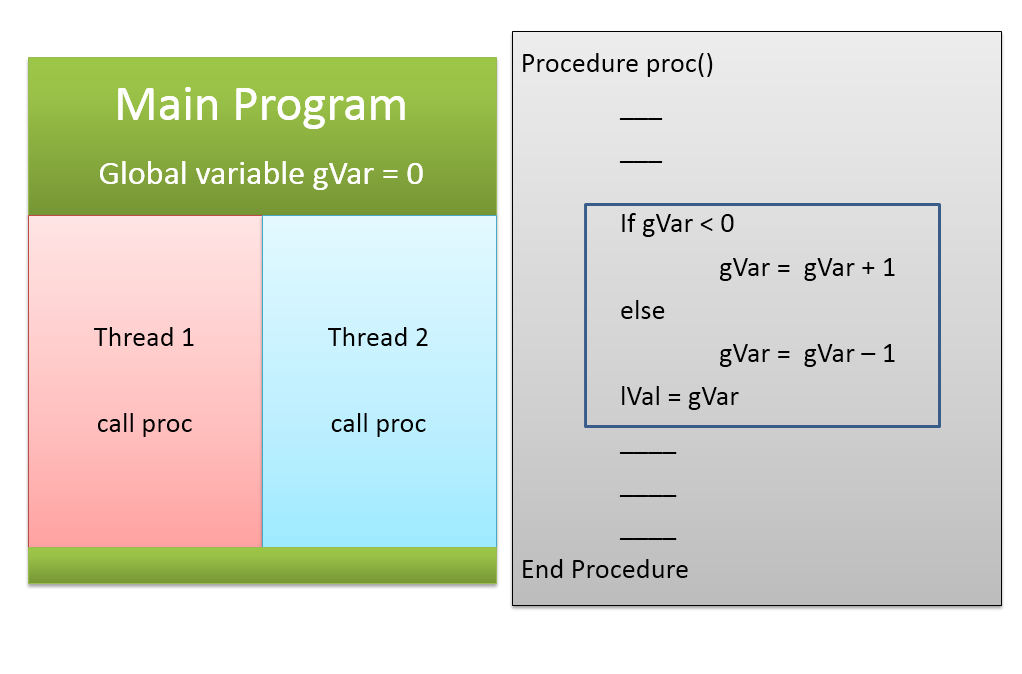
\includegraphics[scale=0.5]{critical_section.png}
\caption{Critical Section}
\label{<<Label>>}
\end{figure}
\paragraph{}
In the figure shown above, 'gVar' is a global variable of the procedure proc(). Procedure is associated with two threads i.e. Thread1 and Thread2. Now, when execution starts both threads may access the global variable 'gVar' concurrently, hence 'gVar' is a Critical Section for the given procedure.

\subsection{Race Condition}
Race conditions arise in software when separate processes or threads of execution depend on some shared state. Operations upon shared states are critical sections that must be mutually exclusive. Failure to do so opens up the possibility of corrupting the shared state.

Race conditions are notoriously difficult to reproduce and debug, since the end result is nondeterministic, and highly dependent on the relative timing between interfering threads. Problems occurring in production systems can therefore disappear when running in debug mode, when additional logging is added, or when attaching a debugger, often referred to as a Heisenbug. It is therefore highly preferable to avoid race conditions in the first place by careful software design than to fix problems afterwards.

Race conditions occur especially in multithreaded, concurrent, parallel or distributed programs [9].
\begin{figure}[H]
\centering
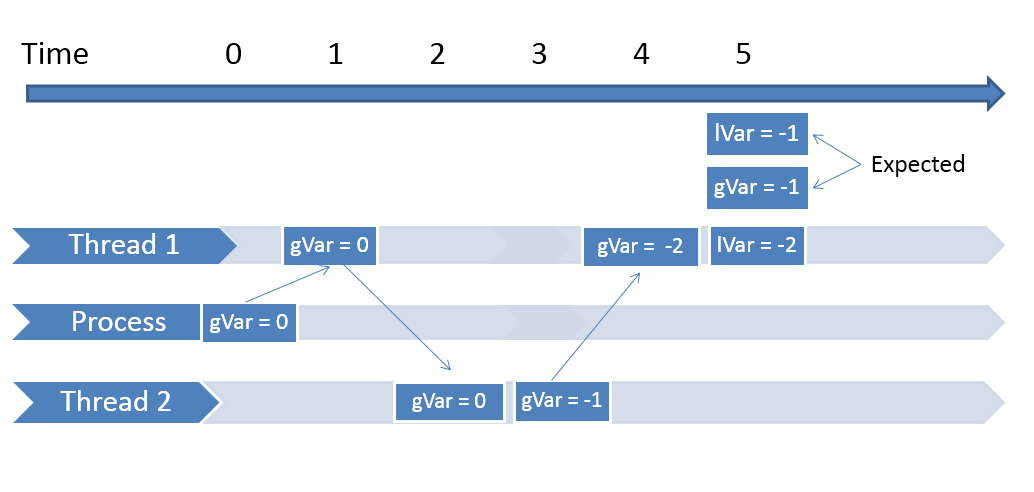
\includegraphics[scale=0.5]{race_condition.png}
\caption{Race Condition}
\label{<<Label>>}
\end{figure}
\paragraph{}
By considering the code snipest shown in fig 1.1: Critical Section, one possible case of execution is shown above in the figure of Race Condition. 
\subsection{Synchronization}

Thread synchronization or serialization, strictly defined, is the application of particular mechanisms to ensure that two concurrently-executing threads or processes do not execute specific portions of a program at the same time. If one thread has begun to execute a serialized portion of the program, any other thread trying to execute this portion must wait until the first thread finishes.

Synchronization is used to control access to state in smallscale multiprocessing systems - in multithreaded environments and multiprocessor computers - and in distributed computers consisting of thousands of units [9].
\begin{figure}[H]
\centering
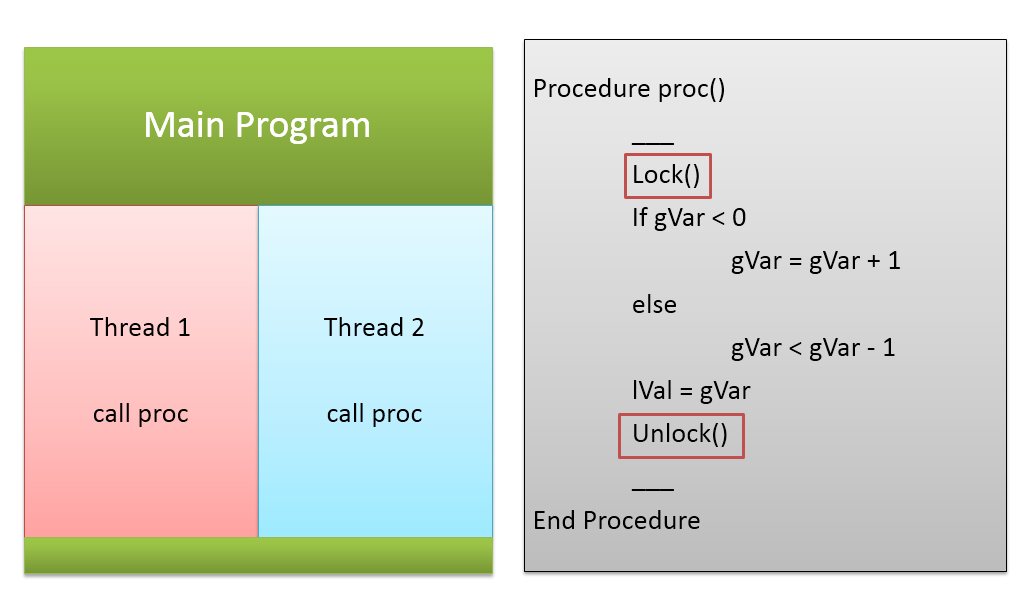
\includegraphics[scale=0.5]{synch.png}
\caption{Synchronization}
\label{<<Label>>}
\end{figure}
\paragraph{}
To avoid the race condition, synchronization mechanism is used in multi threaded programming.Synchronization mechanism may depend on the application logic, hence it differe in many cases.
\section{Need}
When large multithreaded programs are written, its difficult to keep a track of the critical sections in it. This may inturn lead to the occurence of unexpected results or may lead to synchronization bugs. Our project aims to find out these critical sections and introduce a locking mechanism to avoid race conditions in the program[9].

And current version of GCC does not provide or support any feature to find out the critical sections or synchronization bugs in the multitheaded programming.

\section{Motivation}


Motivation behind Critical Section Detection tool is contribution to open source technology, because now a days there are many technologies which are there already implemented based on GCC or Open Source technologies but each of them was developed considering different parameters in front of them. 

Our system is motivated not only considering detecting critical sections but different parameter which are mandatory now a day, like initially we are checking for error free C source code and after that tokenizing and parsing the same source code. So it seems that we need to study all the phases compiler in details and as fat our knowledge about GCC concerns, GCC doesn't provide this featue of detecting critical sections for given source code.

GCC Extension for detecting Critical Sections in a Multi threaded Environment is motivated with respect to many parameter under one basic idea, considering one scenario where one peraon have written a lorge multithreaded code say 1 KLOC and another person tries to work on the same code but unfortunately there are some synchronization bugs, so in such a case it is so difficult to new person to browse that code and detect the suspected critical section or race condiiton. Hence if the tool that we have developed is used by that new person, would become very easy to detect suspected critical section.\\

\section{Objective}
To develop a GCC Extension for detecting Critical Sections and providing locking and unlocking mechanism or synchronization mechanism which may lead to race Condition or Synchronization bugs in a Multithreaded Environment.

The main objective of the system is, the tool should automatically detect the suspected critical sections which may lead to race conditions or synchronization bugs in a multitheaded program.

